\section{Worker scaling}
Our domain decomposition recognizes that account actions are ``embarassingly parallel'' since accounts never interact with each other.
Scaling to accommodate more users is as straightforward as adding more workers.

\subsection{The sixty second golden window}
Many of the business logic requirements inherit time limitations from the sixty second validity window for a quote.
Therefore, if an entire workload can be completed in under sixty seconds then all quotes are valid for the entire run.
This gives rise to a ``golden window'' of performance where workloads that complete in within the window have drastically higher TPS than those that miss the window.

\begin{figure}[tbph]
  \centering
  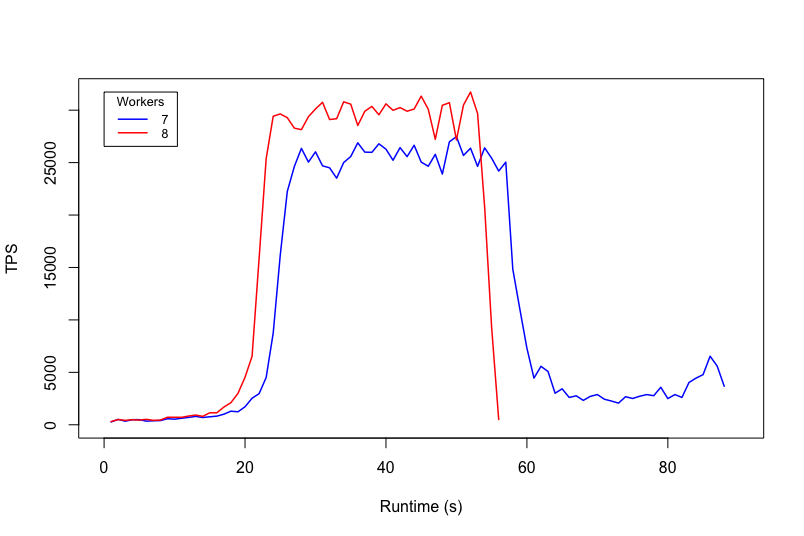
\includegraphics[width=0.7\linewidth]{../graphics/7v8}
  \caption[The golden window effect on TPS]{1000 user workload: 8 Workers, 18k average TPS; 7 Workers, 10k average TPS}
  \label{fig:tps-window}
\end{figure}

Even though approximately 90\% of the commands are completed in 60 seconds by seven workers in Figure~\ref{fig:tps-window}, the remaining 10\% need new quotes and the retrieval delay adds over 50\% to the total runtime.
The penalty for missing the golden window is severe.

\subsection{Scaling results}\label{sec:worker-scaling-results}
The 1000 user workload was used to test the effect of increasing the number of workers.
Figure~\ref{fig:tps-scaling} shows that increasing the number of workers decreases the total time to retrieve quotes, increases the maximum TPS and decreases the total runtime.

\begin{figure}[tbph]
  \centering
  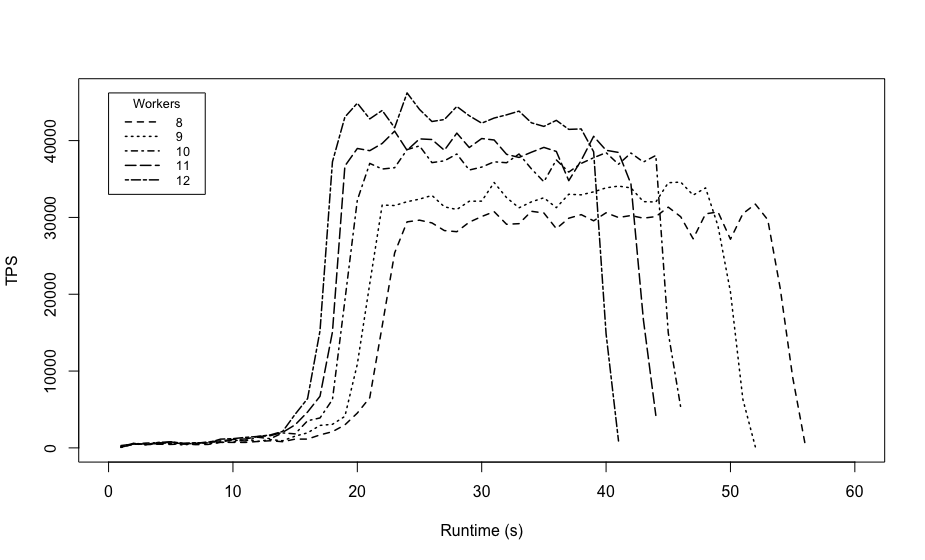
\includegraphics[width=0.8\linewidth]{../graphics/multi-worker}
  \caption{Scaling workers for 1000 user workload}
  \label{fig:tps-scaling}
\end{figure}

With twelve workers we achieved a maximum 26.1k average TPS for the 1000 user workload and a peak TPS over 45k. (See~\ref{sec:starvation} for why we did not add more workers.)

There are two distinct modes of operation for the system: quote-fetching and nominal\footnote{Specifically, the system is at ``nominal TPS'' when it is within 85\% of max TPS.} operation.
During quote-fetching, transactions in workers generate local quote cache misses and are blocked on responses from the quote manager.
During nominal operation the workers have a full set of quotes cached locally and no longer have to block on responses from network services.
The jaggedness in the nominal TPS region is noise from plotting a single run with each worker configuration.

The average TPS value during nominal operation indicates weak linear scaling with the number of workers.
Again, repeated runs should decrease the error.

\begin{figure}[tbph]
  \centering
  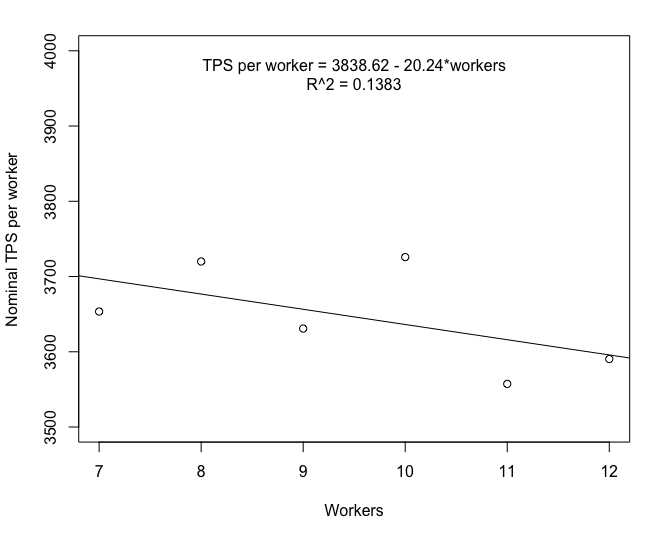
\includegraphics[width=0.7\linewidth]{graphics/tps-per-worker}
  \caption{TPS scaling with workers for 1000 user workload}
  \label{fig:tps-per-worker}
\end{figure}

It's important to note that even when runtime exceeds the golden window the nominal operation speed of the workers is relatively constant.
This indicates that successful methods for scaling the application will involve decreasing the time to reach nominal TPS and then adding more workers.
Chapter~\ref{ch:cap} documents our efforts to realize this scaling.

